
%% bare_adv.tex
%% V1.4b
%% 2015/08/26
%% by Michael Shell
%% See: 
%% http://www.michaelshell.org/
%% for current contact information.
%%
%% This is a skeleton file demonstrating the advanced use of IEEEtran.cls
%% (requires IEEEtran.cls version 1.8b or later) with an IEEE Computer
%% Society journal paper.
%%
%% Support sites:
%% http://www.michaelshell.org/tex/ieeetran/
%% http://www.ctan.org/pkg/ieeetran
%% and
%% http://www.ieee.org/

%%*************************************************************************
%% Legal Notice:
%% This code is offered as-is without any warranty either expressed or
%% implied; without even the implied warranty of MERCHANTABILITY or
%% FITNESS FOR A PARTICULAR PURPOSE! 
%% User assumes all risk.
%% In no event shall the IEEE or any contributor to this code be liable for
%% any damages or losses, including, but not limited to, incidental,
%% consequential, or any other damages, resulting from the use or misuse
%% of any information contained here.
%%
%% All comments are the opinions of their respective authors and are not
%% necessarily endorsed by the IEEE.
%%
%% This work is distributed under the LaTeX Project Public License (LPPL)
%% ( http://www.latex-project.org/ ) version 1.3, and may be freely used,
%% distributed and modified. A copy of the LPPL, version 1.3, is included
%% in the base LaTeX documentation of all distributions of LaTeX released
%% 2003/12/01 or later.
%% Retain all contribution notices and credits.
%% ** Modified files should be clearly indicated as such, including  **
%% ** renaming them and changing author support contact information. **
%%*************************************************************************


% *** Authors should verify (and, if needed, correct) their LaTeX system  ***
% *** with the testflow diagnostic prior to trusting their LaTeX platform ***
% *** with production work. The IEEE's font choices and paper sizes can   ***
% *** trigger bugs that do not appear when using other class files.       ***
% The testflow support page is at:
% http://www.michaelshell.org/tex/testflow/






\documentclass[10pt,journal,compsoc]{IEEEtran}

% *** CITATION PACKAGES ***
%
\ifCLASSOPTIONcompsoc
  % The IEEE Computer Society needs nocompress option
  % requires cite.sty v4.0 or later (November 2003)
  \usepackage[nocompress]{cite}
\else
  % normal IEEE
  \usepackage{cite}
\fi
% cite.sty was written by Donald Arseneau
% V1.6 and later of IEEEtran pre-defines the format of the cite.sty package
% \cite{} output to follow that of the IEEE. Loading the cite package will
% result in citation numbers being automatically sorted and properly
% "compressed/ranged". e.g., [1], [9], [2], [7], [5], [6] without using
% cite.sty will become [1], [2], [5]--[7], [9] using cite.sty. cite.sty's
% \cite will automatically add leading space, if needed. Use cite.sty's
% noadjust option (cite.sty V3.8 and later) if you want to turn this off
% such as if a citation ever needs to be enclosed in parenthesis.
% cite.sty is already installed on most LaTeX systems. Be sure and use
% version 5.0 (2009-03-20) and later if using hyperref.sty.
% The latest version can be obtained at:
% http://www.ctan.org/pkg/cite
% The documentation is contained in the cite.sty file itself.
%
% Note that some packages require special options to format as the Computer
% Society requires. In particular, Computer Society  papers do not use
% compressed citation ranges as is done in typical IEEE papers
% (e.g., [1]-[4]). Instead, they list every citation separately in order
% (e.g., [1], [2], [3], [4]). To get the latter we need to load the cite
% package with the nocompress option which is supported by cite.sty v4.0
% and later.





% *** GRAPHICS RELATED PACKAGES ***
%
\ifCLASSINFOpdf
   \usepackage[pdftex]{graphicx}
  % declare the path(s) where your graphic files are
   \graphicspath{{./resources/}}
  % \graphicspath{{../pdf/}{../jpeg/}}
  % and their extensions so you won't have to specify these with
  % every instance of \includegraphics
   \DeclareGraphicsExtensions{.pdf,.jpeg,.png}
\else
  % or other class option (dvipsone, dvipdf, if not using dvips). graphicx
  % will default to the driver specified in the system graphics.cfg if no
  % driver is specified.
  % \usepackage[dvips]{graphicx}
  % declare the path(s) where your graphic files are
  % \graphicspath{{../eps/}}
  % and their extensions so you won't have to specify these with
  % every instance of \includegraphics
  % \DeclareGraphicsExtensions{.eps}
\fi
% graphicx was written by David Carlisle and Sebastian Rahtz. It is
% required if you want graphics, photos, etc. graphicx.sty is already
% installed on most LaTeX systems. The latest version and documentation
% can be obtained at: 
% http://www.ctan.org/pkg/graphicx
% Another good source of documentation is "Using Imported Graphics in
% LaTeX2e" by Keith Reckdahl which can be found at:
% http://www.ctan.org/pkg/epslatex
%
% latex, and pdflatex in dvi mode, support graphics in encapsulated
% postscript (.eps) format. pdflatex in pdf mode supports graphics
% in .pdf, .jpeg, .png and .mps (metapost) formats. Users should ensure
% that all non-photo figures use a vector format (.eps, .pdf, .mps) and
% not a bitmapped formats (.jpeg, .png). The IEEE frowns on bitmapped formats
% which can result in "jaggedy"/blurry rendering of lines and letters as
% well as large increases in file sizes.
%
% You can find documentation about the pdfTeX application at:
% http://www.tug.org/applications/pdftex





% *** MATH PACKAGES ***
%
\usepackage{amsmath}
% A popular package from the American Mathematical Society that provides
% many useful and powerful commands for dealing with mathematics.
%
% Note that the amsmath package sets \interdisplaylinepenalty to 10000
% thus preventing page breaks from occurring within multiline equations. Use:
\interdisplaylinepenalty=2500
% after loading amsmath to restore such page breaks as IEEEtran.cls normally
% does. amsmath.sty is already installed on most LaTeX systems. The latest
% version and documentation can be obtained at:
% http://www.ctan.org/pkg/amsmath





% *** SPECIALIZED LIST PACKAGES ***
%\usepackage{acronym}
% acronym.sty was written by Tobias Oetiker. This package provides tools for
% managing documents with large numbers of acronyms. (You don't *have* to
% use this package - unless you have a lot of acronyms, you may feel that
% such package management of them is bit of an overkill.)
% Do note that the acronym environment (which lists acronyms) will have a
% problem when used under IEEEtran.cls because acronym.sty relies on the
% description list environment - which IEEEtran.cls has customized for
% producing IEEE style lists. A workaround is to declared the longest
% label width via the IEEEtran.cls \IEEEiedlistdecl global control:
%
% \renewcommand{\IEEEiedlistdecl}{\IEEEsetlabelwidth{SONET}}
% \begin{acronym}
%
% \end{acronym}
% \renewcommand{\IEEEiedlistdecl}{\relax}% remember to reset \IEEEiedlistdecl
%
% instead of using the acronym environment's optional argument.
% The latest version and documentation can be obtained at:
% http://www.ctan.org/pkg/acronym

\usepackage{algorithm}
\usepackage{algorithmic}
% algorithmic.sty was written by Peter Williams and Rogerio Brito.
% This package provides an algorithmic environment for describing algorithms.
% You can use the algorithmic environment in-text or within a figure
% environment to provide for a floating algorithm. Do NOT use the algorithm
% floating environment provided by algorithm.sty (by the same authors) or
% algorithm2e.sty (by Christophe Fiorio) as the IEEE does not use dedicated
% algorithm float types and packages that provide these will not provide
% correct IEEE style captions. The latest version and documentation of
% algorithmic.sty can be obtained at:
% http://www.ctan.org/pkg/algorithms
% Also of interest may be the (relatively newer and more customizable)
% algorithmicx.sty package by Szasz Janos:
% http://www.ctan.org/pkg/algorithmicx




% *** ALIGNMENT PACKAGES ***
%
%\usepackage{array}
% Frank Mittelbach's and David Carlisle's array.sty patches and improves
% the standard LaTeX2e array and tabular environments to provide better
% appearance and additional user controls. As the default LaTeX2e table
% generation code is lacking to the point of almost being broken with
% respect to the quality of the end results, all users are strongly
% advised to use an enhanced (at the very least that provided by array.sty)
% set of table tools. array.sty is already installed on most systems. The
% latest version and documentation can be obtained at:
% http://www.ctan.org/pkg/array


%\usepackage{mdwmath}
%\usepackage{mdwtab}
% Also highly recommended is Mark Wooding's extremely powerful MDW tools,
% especially mdwmath.sty and mdwtab.sty which are used to format equations
% and tables, respectively. The MDWtools set is already installed on most
% LaTeX systems. The lastest version and documentation is available at:
% http://www.ctan.org/pkg/mdwtools


% IEEEtran contains the IEEEeqnarray family of commands that can be used to
% generate multiline equations as well as matrices, tables, etc., of high
% quality.


%\usepackage{eqparbox}
% Also of notable interest is Scott Pakin's eqparbox package for creating
% (automatically sized) equal width boxes - aka "natural width parboxes".
% Available at:
% http://www.ctan.org/pkg/eqparbox




% *** SUBFIGURE PACKAGES ***
%\ifCLASSOPTIONcompsoc
%  \usepackage[caption=false,font=footnotesize,labelfont=sf,textfont=sf]{subfig}
%\else
%  \usepackage[caption=false,font=footnotesize]{subfig}
%\fi
% subfig.sty, written by Steven Douglas Cochran, is the modern replacement
% for subfigure.sty, the latter of which is no longer maintained and is
% incompatible with some LaTeX packages including fixltx2e. However,
% subfig.sty requires and automatically loads Axel Sommerfeldt's caption.sty
% which will override IEEEtran.cls' handling of captions and this will result
% in non-IEEE style figure/table captions. To prevent this problem, be sure
% and invoke subfig.sty's "caption=false" package option (available since
% subfig.sty version 1.3, 2005/06/28) as this is will preserve IEEEtran.cls
% handling of captions.
% Note that the Computer Society format requires a sans serif font rather
% than the serif font used in traditional IEEE formatting and thus the need
% to invoke different subfig.sty package options depending on whether
% compsoc mode has been enabled.
%
% The latest version and documentation of subfig.sty can be obtained at:
% http://www.ctan.org/pkg/subfig




% *** FLOAT PACKAGES ***
%
%\usepackage{fixltx2e}
% fixltx2e, the successor to the earlier fix2col.sty, was written by
% Frank Mittelbach and David Carlisle. This package corrects a few problems
% in the LaTeX2e kernel, the most notable of which is that in current
% LaTeX2e releases, the ordering of single and double column floats is not
% guaranteed to be preserved. Thus, an unpatched LaTeX2e can allow a
% single column figure to be placed prior to an earlier double column
% figure.
% Be aware that LaTeX2e kernels dated 2015 and later have fixltx2e.sty's
% corrections already built into the system in which case a warning will
% be issued if an attempt is made to load fixltx2e.sty as it is no longer
% needed.
% The latest version and documentation can be found at:
% http://www.ctan.org/pkg/fixltx2e


%\usepackage{stfloats}
% stfloats.sty was written by Sigitas Tolusis. This package gives LaTeX2e
% the ability to do double column floats at the bottom of the page as well
% as the top. (e.g., "\begin{figure*}[!b]" is not normally possible in
% LaTeX2e). It also provides a command:
%\fnbelowfloat
% to enable the placement of footnotes below bottom floats (the standard
% LaTeX2e kernel puts them above bottom floats). This is an invasive package
% which rewrites many portions of the LaTeX2e float routines. It may not work
% with other packages that modify the LaTeX2e float routines. The latest
% version and documentation can be obtained at:
% http://www.ctan.org/pkg/stfloats
% Do not use the stfloats baselinefloat ability as the IEEE does not allow
% \baselineskip to stretch. Authors submitting work to the IEEE should note
% that the IEEE rarely uses double column equations and that authors should try
% to avoid such use. Do not be tempted to use the cuted.sty or midfloat.sty
% packages (also by Sigitas Tolusis) as the IEEE does not format its papers in
% such ways.
% Do not attempt to use stfloats with fixltx2e as they are incompatible.
% Instead, use Morten Hogholm'a dblfloatfix which combines the features
% of both fixltx2e and stfloats:
%
% \usepackage{dblfloatfix}
% The latest version can be found at:
% http://www.ctan.org/pkg/dblfloatfix


%\ifCLASSOPTIONcaptionsoff
%  \usepackage[nomarkers]{endfloat}
% \let\MYoriglatexcaption\caption
% \renewcommand{\caption}[2][\relax]{\MYoriglatexcaption[#2]{#2}}
%\fi
% endfloat.sty was written by James Darrell McCauley, Jeff Goldberg and 
% Axel Sommerfeldt. This package may be useful when used in conjunction with 
% IEEEtran.cls'  captionsoff option. Some IEEE journals/societies require that
% submissions have lists of figures/tables at the end of the paper and that
% figures/tables without any captions are placed on a page by themselves at
% the end of the document. If needed, the draftcls IEEEtran class option or
% \CLASSINPUTbaselinestretch interface can be used to increase the line
% spacing as well. Be sure and use the nomarkers option of endfloat to
% prevent endfloat from "marking" where the figures would have been placed
% in the text. The two hack lines of code above are a slight modification of
% that suggested by in the endfloat docs (section 8.4.1) to ensure that
% the full captions always appear in the list of figures/tables - even if
% the user used the short optional argument of \caption[]{}.
% IEEE papers do not typically make use of \caption[]'s optional argument,
% so this should not be an issue. A similar trick can be used to disable
% captions of packages such as subfig.sty that lack options to turn off
% the subcaptions:
% For subfig.sty:
% \let\MYorigsubfloat\subfloat
% \renewcommand{\subfloat}[2][\relax]{\MYorigsubfloat[]{#2}}
% However, the above trick will not work if both optional arguments of
% the \subfloat command are used. Furthermore, there needs to be a
% description of each subfigure *somewhere* and endfloat does not add
% subfigure captions to its list of figures. Thus, the best approach is to
% avoid the use of subfigure captions (many IEEE journals avoid them anyway)
% and instead reference/explain all the subfigures within the main caption.
% The latest version of endfloat.sty and its documentation can obtained at:
% http://www.ctan.org/pkg/endfloat
%
% The IEEEtran \ifCLASSOPTIONcaptionsoff conditional can also be used
% later in the document, say, to conditionally put the References on a 
% page by themselves.





% *** PDF, URL AND HYPERLINK PACKAGES ***
%
%\usepackage{url}
% url.sty was written by Donald Arseneau. It provides better support for
% handling and breaking URLs. url.sty is already installed on most LaTeX
% systems. The latest version and documentation can be obtained at:
% http://www.ctan.org/pkg/url
% Basically, \url{my_url_here}.


% NOTE: PDF thumbnail features are not required in IEEE papers
%       and their use requires extra complexity and work.
%\ifCLASSINFOpdf
%  \usepackage[pdftex]{thumbpdf}
%\else
%  \usepackage[dvips]{thumbpdf}
%\fi
% thumbpdf.sty and its companion Perl utility were written by Heiko Oberdiek.
% It allows the user a way to produce PDF documents that contain fancy
% thumbnail images of each of the pages (which tools like acrobat reader can
% utilize). This is possible even when using dvi->ps->pdf workflow if the
% correct thumbpdf driver options are used. thumbpdf.sty incorporates the
% file containing the PDF thumbnail information (filename.tpm is used with
% dvips, filename.tpt is used with pdftex, where filename is the base name of
% your tex document) into the final ps or pdf output document. An external
% utility, the thumbpdf *Perl script* is needed to make these .tpm or .tpt
% thumbnail files from a .ps or .pdf version of the document (which obviously
% does not yet contain pdf thumbnails). Thus, one does a:
% 
% thumbpdf filename.pdf 
%
% to make a filename.tpt, and:
%
% thumbpdf --mode dvips filename.ps
%
% to make a filename.tpm which will then be loaded into the document by
% thumbpdf.sty the NEXT time the document is compiled (by pdflatex or
% latex->dvips->ps2pdf). Users must be careful to regenerate the .tpt and/or
% .tpm files if the main document changes and then to recompile the
% document to incorporate the revised thumbnails to ensure that thumbnails
% match the actual pages. It is easy to forget to do this!
% 
% Unix systems come with a Perl interpreter. However, MS Windows users
% will usually have to install a Perl interpreter so that the thumbpdf
% script can be run. The Ghostscript PS/PDF interpreter is also required.
% See the thumbpdf docs for details. The latest version and documentation
% can be obtained at.
% http://www.ctan.org/pkg/thumbpdf


% NOTE: PDF hyperlink and bookmark features are not required in IEEE
%       papers and their use requires extra complexity and work.
% *** IF USING HYPERREF BE SURE AND CHANGE THE EXAMPLE PDF ***
% *** TITLE/SUBJECT/AUTHOR/KEYWORDS INFO BELOW!!           ***
\newcommand\MYhyperrefoptions{
    bookmarks=true,
    bookmarksnumbered=true,
    pdfpagemode={UseOutlines},
    plainpages=false,
    pdfpagelabels=true,
    colorlinks=true,
    linkcolor={black},
    citecolor={black},
    urlcolor={black},
    pdftitle={A0209166A},%<!CHANGE!
% pdfsubject={Cryptography},%<!CHANGE!
% pdfauthor={SHEN Jiamin},%<!CHANGE!
% pdfkeywords={}
}%<^!CHANGE!
%\ifCLASSINFOpdf
%\usepackage[\MYhyperrefoptions,pdftex]{hyperref}
%\else
%\usepackage[\MYhyperrefoptions,breaklinks=true,dvips]{hyperref}
%\usepackage{breakurl}
%\fi
% One significant drawback of using hyperref under DVI output is that the
% LaTeX compiler cannot break URLs across lines or pages as can be done
% under pdfLaTeX's PDF output via the hyperref pdftex driver. This is
% probably the single most important capability distinction between the
% DVI and PDF output. Perhaps surprisingly, all the other PDF features
% (PDF bookmarks, thumbnails, etc.) can be preserved in
% .tex->.dvi->.ps->.pdf workflow if the respective packages/scripts are
% loaded/invoked with the correct driver options (dvips, etc.). 
% As most IEEE papers use URLs sparingly (mainly in the references), this
% may not be as big an issue as with other publications.
%
% That said, Vilar Camara Neto created his breakurl.sty package which
% permits hyperref to easily break URLs even in dvi mode.
% Note that breakurl, unlike most other packages, must be loaded
% AFTER hyperref. The latest version of breakurl and its documentation can
% be obtained at:
% http://www.ctan.org/pkg/breakurl
% breakurl.sty is not for use under pdflatex pdf mode.
%
% The advanced features offer by hyperref.sty are not required for IEEE
% submission, so users should weigh these features against the added
% complexity of use.
% The package options above demonstrate how to enable PDF bookmarks
% (a type of table of contents viewable in Acrobat Reader) as well as
% PDF document information (title, subject, author and keywords) that is
% viewable in Acrobat reader's Document_Properties menu. PDF document
% information is also used extensively to automate the cataloging of PDF
% documents. The above set of options ensures that hyperlinks will not be
% colored in the text and thus will not be visible in the printed page,
% but will be active on "mouse over". USING COLORS OR OTHER HIGHLIGHTING
% OF HYPERLINKS CAN RESULT IN DOCUMENT REJECTION BY THE IEEE, especially if
% these appear on the "printed" page. IF IN DOUBT, ASK THE RELEVANT
% SUBMISSION EDITOR. You may need to add the option hypertexnames=false if
% you used duplicate equation numbers, etc., but this should not be needed
% in normal IEEE work.
% The latest version of hyperref and its documentation can be obtained at:
% http://www.ctan.org/pkg/hyperref



\usepackage{minted}



% *** Do not adjust lengths that control margins, column widths, etc. ***
% *** Do not use packages that alter fonts (such as pslatex).         ***
% There should be no need to do such things with IEEEtran.cls V1.6 and later.
% (Unless specifically asked to do so by the journal or conference you plan
% to submit to, of course. )


% correct bad hyphenation here
\hyphenation{op-tical net-works semi-conduc-tor}


\begin{document}
%
% paper title
% Titles are generally capitalized except for words such as a, an, and, as,
% at, but, by, for, in, nor, of, on, or, the, to and up, which are usually
% not capitalized unless they are the first or last word of the title.
% Linebreaks \\ can be used within to get better formatting as desired.
% Do not put math or special symbols in the title.
\title{Assignment 2 - PART I}

\author{SHEN~Jiamin 
    \thanks{\textbf{SHEN Jiamin}} 
    \thanks{Student ID: A0209166A} 
    \thanks{NUSNET ID: E0446373} 
    \thanks{\texttt{shen\_jiamin@comp.nus.edu.sg}}
}

% The paper headers
\markboth{CS4236 - Cryptography Theory and Practice}{SHEN Jiamin - A0209166A}

% make the title area
\maketitle

\section{Secret Key Encryption}

%%%%%%%%%%%%%%%%%%%%%%%%%%%%%%%%%%%%%%%%%%%%%%%%%%%%%%%%%%%%%%%%%%%%%%%%%%%%%%%%
\subsection{Encryption using Different Ciphers and Modes}

For this section, I used 3 different ciphers in different modes. 
They are
\begin{enumerate}
    \item Block cipher AES in CFB mode, where key length is 256.
    \item Block cipher SM4 in CTR mode.
    \item Stream cipher RC4.
\end{enumerate}%

Commands used is screenshot as Fig.\ref{fig:p1_1}:

\begin{figure}[hb]
\centering
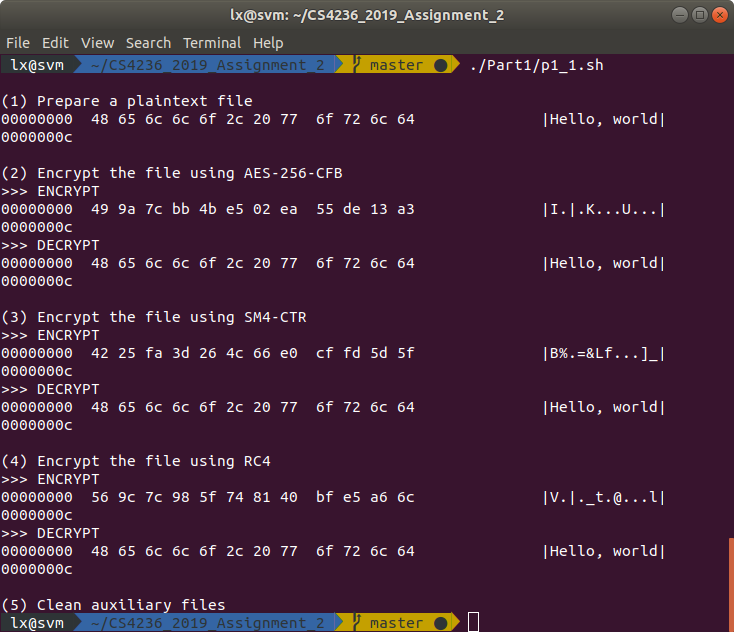
\includegraphics[width=\columnwidth]{resources/p1_1.png}
\caption{
    Content in file \texttt{Part1/p1\_1.sh} is listed in Appendix \ref{code:1_1}
}
\label{fig:p1_1}
\end{figure}

%%%%%%%%%%%%%%%%%%%%%%%%%%%%%%%%%%%%%%%%%%%%%%%%%%%%%%%%%%%%%%%%%%%%%%%%%%%%%%%%
\subsection{Encryption Mode – ECB vs. CBC}

\begin{figure}[t!]
\centering
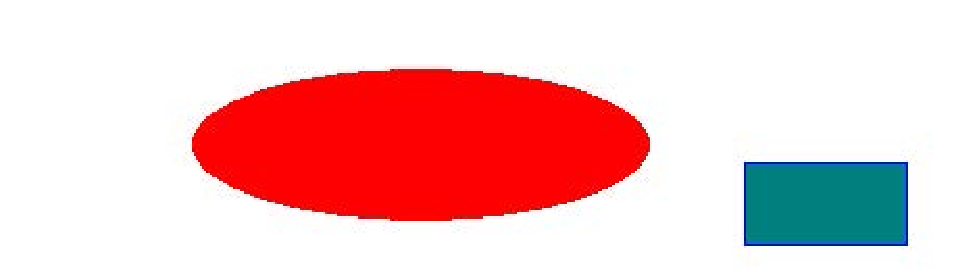
\includegraphics[width=\columnwidth]{resources/pic_original.pdf}
\caption{
    The original picture
}
\label{fig:pic_original}
\end{figure}

\begin{figure}[t!]
\centering
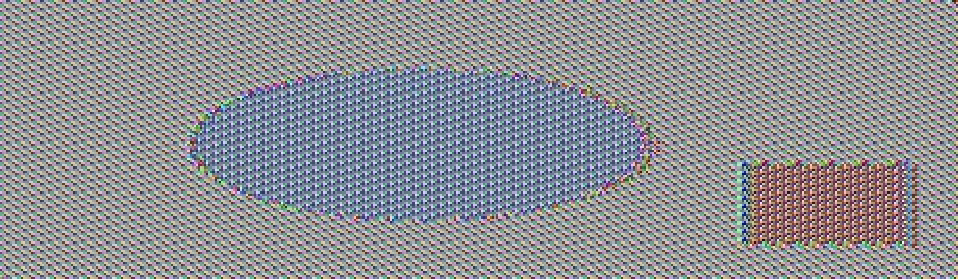
\includegraphics[width=\columnwidth]{resources/pic_ecb.pdf}
\caption{
    The picture encrypted in ECB mode.
}
\label{fig:pic_ecb}
\end{figure}

\begin{figure}[t!]
\centering

\includegraphics[width=\columnwidth]{resources/pic_cbc.pdf}
\caption{
    The picture encrypted in CBC mode.
}
\label{fig:pic_cbc}
\end{figure}

From the ECB-encrypted picture (Fig.\ref{fig:pic_ecb}), we can clearly see the edges of the graphics.
While from the CBC-encrypted picture (Fig.\ref{fig:pic_cbc}), we can hardly find any information.

Using ECB mode merely concatenates the output of the block cipher as the ciphertext. 
That is, the same blocks of plaintext was mapped to the same ciphertext.
We don't change the relative position of blocks either. Consequently, the shape information was almost completely preserved. 

In CBC mode, each block of plaintext is firstly XOR-ed with the previous block of ciphertext. Therefore, identical blocks are encoded as different ciphertext. So the shape information was well hidden. 

%%%%%%%%%%%%%%%%%%%%%%%%%%%%%%%%%%%%%%%%%%%%%%%%%%%%%%%%%%%%%%%%%%%%%%%%%%%%%%%%
\subsection{Initialization Vector (IV)}

\subsubsection{}

Screenshot of the commands and outputs is as Fig.\ref{fig:p1_3_1}.

\begin{figure}[t!]
\centering
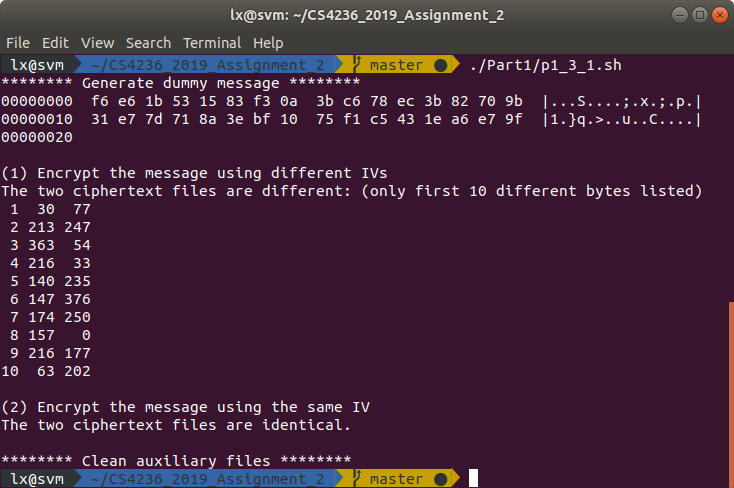
\includegraphics[width=\columnwidth]{resources/p1_3_1.png}
\caption{
    Content in file \texttt{Part1/p1\_3\_1.sh} is listed in Appendix \ref{code:1_3_1}
}
\label{fig:p1_3_1}
\end{figure}

From the outputs, it can be seen that reusing IV under the same key to encrypt the same message leads to the same ciphertext.

CPA-security requires that the encryption scheme should be probabilistic. 
A probabilistic function has to be able to get access to a randomness source.
In the encryption schemes we used, IV is the only source of randomness.
Hence if we reuse the IV, the probabilistic function falls back to a deterministic function.

Therefore, in order to keep the encryption scheme produces different ciphertext for the same plaintext, IV can never be reused.

\subsubsection{}
Yes, he/she can decrypt other messages that are not longer than the known message. Screenshot of the commands and outputs is as Fig.\ref{fig:p1_3_2}.

\begin{figure}[t!]
\centering
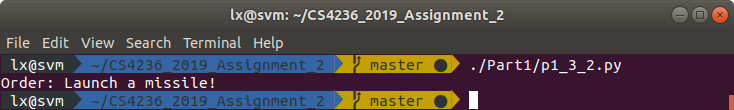
\includegraphics[width=\columnwidth]{resources/p1_3_2.png}
\caption{
    Content in file \texttt{Part1/p1\_3\_2.sh} is listed in Appendix \ref{code:1_3_2}
}
\label{fig:p1_3_2}
\end{figure}

If we use CFB mode (Fig.\ref{fig:CFB_encryption}) instead of OFB mode, we can only get the first block of a new message.

\begin{figure}[ht]
\centering

\includegraphics[width=\columnwidth]{resources/CFB_encryption.png}
\caption{
    Cipher Feedback (CFB) mode encryption \protect\footnotemark
}
\label{fig:CFB_encryption}
\end{figure}

\footnotetext{The picture comes from \texttt{https://bit.ly/1CoRiM0}}

With CFB mode, we can decrypt any message no longer than the known message because CFB generates a completely the same random stream with the same IV and xor the random stream with plaintext.

While in OFB mode, the random stream is generated not only from the IV, but also influenced by the previous block of message. Hence although the IV and the key are the same, it can generate different random stream from different messages.

But we can still get the first block of message because $m_0 \oplus c_0$ always equals to $F_k(IV)$. This is sufficient to win the CPA game.

\subsubsection{}

Screenshot of the commands and outputs is as Fig.\ref{fig:p1_3_3}.

Since the message is shorter than a block, we only consider the message and ciphertext with only one block.
In CBC mode (Fig.\ref{fig:CBC_encryption}), the first block of ciphertext 
$$c := F_k(IV \oplus m)$$
Thus knowing IV, we can keep the ciphertext identical by holding $IV \oplus m$ a constant.

\begin{figure}[t!]
\centering
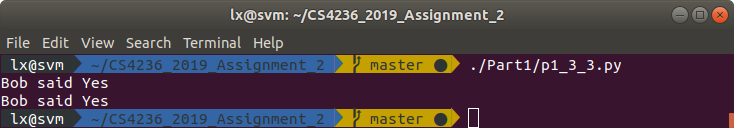
\includegraphics[width=\columnwidth]{resources/p1_3_3.png}
\caption{
    Content in file \texttt{Part1/p1\_3\_3.sh} is listed in Appendix \ref{code:1_3_3}
}
\label{fig:p1_3_3}
\end{figure}

\begin{figure}[ht]
\centering

\includegraphics[width=\columnwidth]{resources/CBC_encryption.png}
\caption{
    Cipher Block Chaining (CBC) mode encryption \protect\footnotemark
}
\label{fig:CBC_encryption}
\end{figure}

\footnotetext{The picture comes from \texttt{https://bit.ly/1CoRiM0}}

To solve this problem, we can keep $IV_1 \oplus m = IV_2 \oplus m'$, where $m$ is \texttt{Yes} or \texttt{No}, $IV_1$ and $IV_2$ are known value. Thus
$$ m' = m \oplus IV_1 \oplus IV_2 $$
can be easily constructed. Then we ask Bob to encrypt the $m'$ and check if the response $C$ equals to the ciphertext $C_1$ we already known. If $C = C_1$, $m$ is exactly the message Bob sent just now.


\section{Public Key Encryption}

Note: all codes in this section include a common header file, \texttt{Part1/p2\_common.h}, which can be found in Appendix \ref{code:2_common}.

%%%%%%%%%%%%%%%%%%%%%%%%%%%%%%%%%%%%%%%%%%%%%%%%%%%%%%%%%%%%%%%%%%%%%%%%%%%%%%%%
% \subsection{Background}
% \subsection{BIGNUM APIs}
\setcounter{subsection}{2}
%%%%%%%%%%%%%%%%%%%%%%%%%%%%%%%%%%%%%%%%%%%%%%%%%%%%%%%%%%%%%%%%%%%%%%%%%%%%%%%%
\subsection{Deriving the Private Key}

The algorithm to derive private exponent $d$ is stated as Algorithm \ref{alg:rsa_pqe_d}.
Command and output is screenshot as Fig.\ref{fig:p2_3}.
Code can be found in Appendix \ref{code:2_3}

\begin{algorithm}
\caption{Calculate private key exponent $d$}
\label{alg:rsa_pqe_d}
\begin{algorithmic}
\STATE \textbf{Input:} Private primes $p$,$q$ and public exponent $e$
\STATE \textbf{Output:} Private exponent $d$

\STATE $ n \gets pq $
\STATE $ \phi(n) \gets (p-1)(q-1) $
\STATE $ d \gets e^{-1} \mod{\phi(n)} $
\RETURN $ d $
\end{algorithmic}
\end{algorithm}

\begin{figure}[t!]
\centering
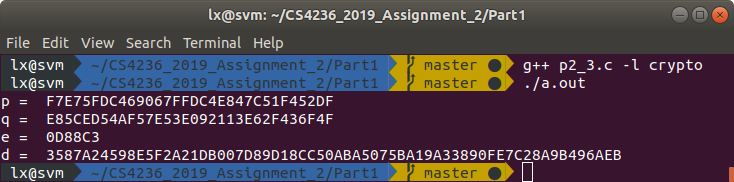
\includegraphics[width=\columnwidth]{resources/p2_3.png}
\caption{
    Calculate private key exponent $d$
}
\label{fig:p2_3}
\end{figure}

%%%%%%%%%%%%%%%%%%%%%%%%%%%%%%%%%%%%%%%%%%%%%%%%%%%%%%%%%%%%%%%%%%%%%%%%%%%%%%%%
\subsection{Encrypting a Message}

The algorithm to encrypt a message $m$ using RSA algorithm with public key $(n, e) $ is stated as Algorithm \ref{alg:rsa_enc}.
Command and output is screenshot as Fig.\ref{fig:p2_4}.
Code can be found in Appendix \ref{code:2_4}

\begin{algorithm}
\caption{RSA encrypt}
\label{alg:rsa_enc}
\begin{algorithmic}
\STATE \textbf{Input:} RSA public key $(n, e)$ and message $m$
\STATE \textbf{Output:} Ciphertext $c$

\STATE $ c \gets m^e \mod{n} $
\RETURN $ c $
\end{algorithmic}
\end{algorithm}

\begin{figure}[ht]
\centering
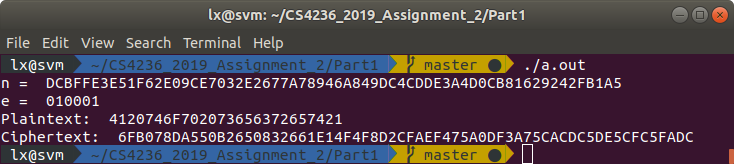
\includegraphics[width=\columnwidth]{resources/p2_4.png}
\caption{
    RSA encrypt
}
\label{fig:p2_4}
\end{figure}

%%%%%%%%%%%%%%%%%%%%%%%%%%%%%%%%%%%%%%%%%%%%%%%%%%%%%%%%%%%%%%%%%%%%%%%%%%%%%%%%
\subsection{Decrypting a Message}

The algorithm to decrypt a ciphertext $c$ using RSA algorithm with private key $(n, d) $ is stated as Algorithm \ref{alg:rsa_dec}.
Command and output is screenshot as Fig.\ref{fig:p2_5}.
Code can be found in Appendix \ref{code:2_5}

\begin{algorithm}
\caption{RSA encrypt}
\label{alg:rsa_dec}
\begin{algorithmic}
\STATE \textbf{Input:} RSA private key $(n, d)$ and ciphertext $c$
\STATE \textbf{Output:} Plaintext $m$

\STATE $ m \gets c^d \mod{n} $
\RETURN $ m $
\end{algorithmic}
\end{algorithm}

\begin{figure}[ht]
\centering
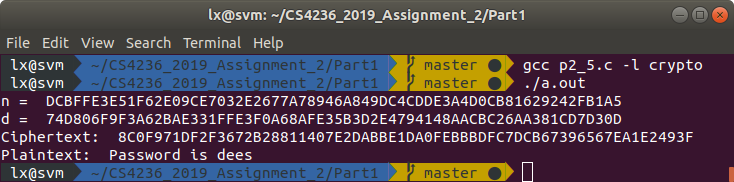
\includegraphics[width=\columnwidth]{resources/p2_5.png}
\caption{
    RSA decrypt
}
\label{fig:p2_5}
\end{figure}

%%%%%%%%%%%%%%%%%%%%%%%%%%%%%%%%%%%%%%%%%%%%%%%%%%%%%%%%%%%%%%%%%%%%%%%%%%%%%%%%
\subsection{Signing a Message}
\label{subs:sign}

The algorithm to sign a message $m$ using RSA algorithm is completely the same as RSA decryption (Algorithm \ref{alg:rsa_dec}) which utilize the private key.
Command and output is screenshot as Fig.\ref{fig:p2_6}.
Code can be found in Appendix \ref{code:2_6}

Note that when I changed \texttt{\$2000} to \texttt{\$3000}, the signature becomes different. Concretely, we changed 1 bit in the message. Then there are 123 different bits (in the total 256 bits) in the two signatures, which is nearly 50\% of all bits.

\begin{figure}[ht]
\centering
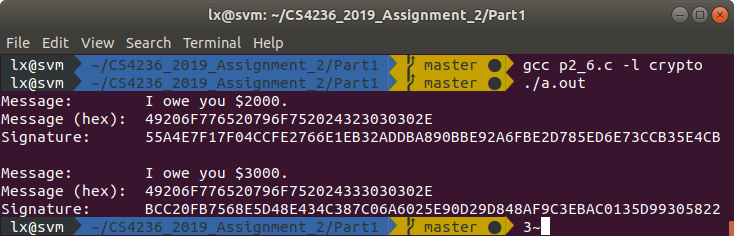
\includegraphics[width=\columnwidth]{resources/p2_6.png}
\caption{
    RSA sign
}
\label{fig:p2_6}
\end{figure}

%%%%%%%%%%%%%%%%%%%%%%%%%%%%%%%%%%%%%%%%%%%%%%%%%%%%%%%%%%%%%%%%%%%%%%%%%%%%%%%%
\subsection{Verifying a Signature}

The algorithm to verify a signature using RSA algorithm is completely the same as RSA encryption (Algorithm \ref{alg:rsa_enc}) which utilize the public key.
Command and output is screenshot as Fig.\ref{fig:p2_7}.
Code can be found in Appendix \ref{code:2_7}

From this example, it can be seen that 1 bit different in the two signature caused the recovered measurements completely different. They even don't have the same length.

This example and the one in Question \ref{subs:sign} show that there's a great diffusion property in RSA.

\begin{figure}[ht]
\centering
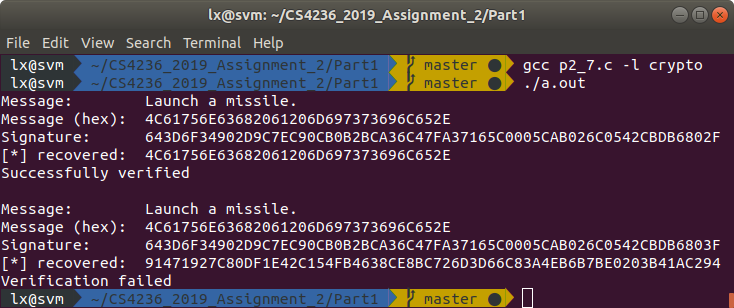
\includegraphics[width=\columnwidth]{resources/p2_7.png}
\caption{
    RSA verify
}
\label{fig:p2_7}
\end{figure}

\newpage
\onecolumn

\appendices

\section{\texttt{Part1/p1\_1.sh}}
\label{code:1_1}
\inputminted{bash}{../Part1/p1_1.sh}
\newpage

\section{\texttt{Part1/p1\_2.sh}}
\label{code:1_2}
\inputminted{bash}{../Part1/p1_2.sh}
\newpage

\section{\texttt{Part1/p1\_3\_1.sh}}
\label{code:1_3_1}
\inputminted{bash}{../Part1/p1_3_1.sh}
\newpage

\section{\texttt{Part1/p1\_3\_2.py}}
\label{code:1_3_2}
\inputminted{python}{../Part1/p1_3_2.py}
\newpage

\section{\texttt{Part1/p1\_3\_3.py}}
\label{code:1_3_3}
\inputminted{python}{../Part1/p1_3_3.py}
\newpage

\section{\texttt{Part1/p2\_common.h}}
\label{code:2_common}
\inputminted{c}{../Part1/p2_common.h}
\newpage

\section{\texttt{Part1/p2\_3.c}}
\label{code:2_3}
\inputminted{c}{../Part1/p2_3.c}
\newpage

\section{\texttt{Part1/p2\_4.c}}
\label{code:2_4}
\inputminted{c}{../Part1/p2_4.c}
\newpage

\section{\texttt{Part1/p2\_5.c}}
\label{code:2_5}
\inputminted{c}{../Part1/p2_5.c}
\newpage

\section{\texttt{Part1/p2\_6.c}}
\label{code:2_6}
\inputminted{c}{../Part1/p2_6.c}
\newpage

\section{\texttt{Part1/p2\_7.c}}
\label{code:2_7}
\inputminted{c}{../Part1/p2_7.c}


% \section{Conclusion}
% The conclusion goes \cite{IEEEhowto:kopka} here.





% references section

% can use a bibliography generated by BibTeX as a .bbl file
% BibTeX documentation can be easily obtained at:
% http://mirror.ctan.org/biblio/bibtex/contrib/doc/
% The IEEEtran BibTeX style support page is at:
% http://www.michaelshell.org/tex/ieeetran/bibtex/
% \bibliographystyle{IEEEtran}
% argument is your BibTeX string definitions and bibliography database(s)
%\bibliography{IEEEabrv,../bib/paper}
%
% <OR> manually copy in the resultant .bbl file
% set second argument of \begin to the number of references
% (used to reserve space for the reference number labels box)
% \begin{thebibliography}{1}

% \bibitem{IEEEhowto:kopka}
% H.~Kopka and P.~W. Daly, \emph{A Guide to {\LaTeX}}, 3rd~ed.\hskip 1em plus
%   0.5em minus 0.4em\relax Harlow, England: Addison-Wesley, 1999.

% \end{thebibliography}


\end{document}


